\documentclass[aspectratio=169]{beamer}
\usepackage{tikz}
\usepackage{booktabs}
\usepackage{xcolor}
\usetikzlibrary{mindmap}

\usetheme{Madrid}
\usecolortheme{beaver}
\setbeamertemplate{navigation symbols}{}

\title{Simone de Beauvoir's Ethics}
\subtitle{An Introduction for Beginning Students}
\author{Brendan Shea, PhD}
\date{Intro to Ethics}

\begin{document}
	
	\begin{frame}
		\titlepage
	\end{frame}
	
	% Slide 1
	\begin{frame}
		\frametitle{Simone de Beauvoir: A Life of Philosophical Engagement (1908-1986)}
		\begin{itemize}
			\item Simone de Beauvoir was born in Paris to a middle-class family and became one of the most influential philosophers of the 20th century.
			\item She attended the Sorbonne where she studied philosophy and met Jean-Paul Sartre, beginning a lifelong intellectual partnership.
			\item De Beauvoir wrote across many genres including philosophy, novels, essays, and memoirs, using each to explore human freedom and ethics.
			\item She actively engaged in the political struggles of her time, including World War II resistance, decolonization movements, and second-wave feminism.
		\end{itemize}
		
		\begin{alertblock}{Key Works}
			\begin{itemize}
				\item \textit{The Ethics of Ambiguity} (1947) - philosophical treatise on ethics
				\item \textit{The Second Sex} (1949) - groundbreaking feminist analysis
				\item \textit{Memoirs of a Dutiful Daughter} (1958) - first volume of autobiography
			\end{itemize}
		\end{alertblock}
	\end{frame}
	
	% Slide 2
	\begin{frame}
		\frametitle{Early Life and Education: The Making of a Philosopher}
		\begin{itemize}
			\item De Beauvoir received a traditional Catholic education in her early years but rejected religion at age 14, declaring herself an atheist.
			\item She excelled academically, completing her baccalauréat with distinctions in mathematics and philosophy.
			\item At the Sorbonne, she studied philosophy alongside luminaries like Maurice Merleau-Ponty and Claude Lévi-Strauss.
			\item She passed the agrégation in philosophy in 1929, becoming the youngest person ever to pass the highly competitive exam.
		\end{itemize}
		
		\begin{center}
			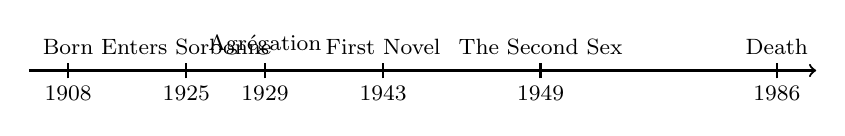
\begin{tikzpicture}
				\scriptsize
				\draw[thick, ->] (0,0) -- (10,0);
				\foreach \x/\year/\event in {
					0.5/1908/Born,
					2/1925/Enters Sorbonne,
					3/1929/Agrégation,
					4.5/1943/First Novel,
					6.5/1949/The Second Sex,
					9.5/1986/Death
				}
				{
					\draw[thick] (\x,-0.1) -- (\x,0.1);
					\node[below] at (\x,-0.1) {\footnotesize \year};
					\node[above] at (\x,0.1) {\footnotesize \event};
				}
			\end{tikzpicture}
		\end{center}
	\end{frame}
	
	% Slide 3
	\begin{frame}
		\frametitle{Intellectual Partnerships: Sartre, Merleau-Ponty, and the Existentialist Circle}
		\begin{itemize}
			\item De Beauvoir and her partner \textbf{Jean Paul Sartre} formed the center of a vibrant intellectual community in Paris, especially at Café de Flore.
			\item Their relationship challenged traditional notions of love and commitment, emphasizing intellectual freedom and honesty.
			\item She maintained important intellectual dialogues with other philosophers including Maurice Merleau-Ponty and Albert Camus.
			\item De Beauvoir was a leading figure in the development of \textbf{existentialist} thought.
		\end{itemize}
		
		\begin{block}{The Existentialist Circle}
			\scriptsize
			Key members of de Beauvoir's intellectual community included:
			\begin{itemize}
				\item Jean-Paul Sartre (philosopher)
				\item Albert Camus (novelist/philosopher) 
				\item Maurice Merleau-Ponty (phenomenologist)
				\item Raymond Aron (sociologist)
			\end{itemize}
		\end{block}
	\end{frame}
	
	% Slide 4
	\begin{frame}
		\frametitle{Writing as Resistance: De Beauvoir During World War II}
		\begin{itemize}
			\item During the Nazi occupation of France, de Beauvoir remained in Paris and continued teaching philosophy.
			\item She joined the French Resistance, though her participation was primarily intellectual rather than in direct combat.
			\item De Beauvoir wrote her first novel \textit{She Came to Stay} (1943) during this period, exploring themes of freedom and interpersonal conflict.
			\item The war experience profoundly shaped her ethical thinking, highlighting questions about individual responsibility during political crisis.
		\end{itemize}
		
		\begin{table}
			\begin{tabular}{ll}
				\toprule
				\textbf{War Experience} & \textbf{Philosophical Impact} \\
				\midrule
				Nazi Occupation & Questioning absolute freedom \\
				Political Resistance & Ethics of engagement \\
				Material Deprivation & Embodied existence \\
				Witnessing Collaboration & Bad faith and responsibility \\
				\bottomrule
			\end{tabular}
			\caption{World War II's Influence on De Beauvoir's Thought}
		\end{table}
	\end{frame}
	
	
	% Slide 5
	\begin{frame}
		\frametitle{Global Impact: Travels, Activism, and Political Engagement}
		\begin{itemize}
			\item After World War II, de Beauvoir traveled extensively, visiting the United States, China, and the Soviet Union.
			\item Her travels informed her political critique of colonialism, particularly evident in her writing about the Algerian War.
			\item She cofounded the journal \textit{Les Temps Modernes} with Sartre, using it as a platform for political and philosophical debate.
			\item In her later years, she became increasingly active in feminist movements, signing the famous Manifesto of the 343 supporting abortion rights.
		\end{itemize}
		
		\begin{columns}
			\begin{column}{0.5\textwidth}
				\textbf{Political Causes:}
				\begin{itemize}
					\item Anti-colonialism
					\item Women's rights
					\item Anti-Vietnam War
					\item Social justice
				\end{itemize}
			\end{column}
			\begin{column}{0.5\textwidth}
				\textbf{Travel Influences:}
				\begin{itemize}
					\item USA (American imperialism)
					\item China (Communism)
					\item USSR (Soviet system)
					\item Algeria (Colonialism)
				\end{itemize}
			\end{column}
		\end{columns}
	\end{frame}
	
	% Slide 6
	\begin{frame}
		\frametitle{Life as Praxis: How de Beauvoir Lived Her Philosophy}
		\begin{itemize}
			\item De Beauvoir rejected traditional marriage and motherhood, living in accordance with her philosophical views on freedom.
			\item She supported herself financially through teaching and writing, maintaining economic independence throughout her life.
			\item Her personal relationships embodied her critique of traditional gender roles and monogamy.
			\item Her later activism for women's rights demonstrated her commitment to moving from theory to practice.
		\end{itemize}
		
		\begin{exampleblock}{Philosophical Praxis in Action}
			De Beauvoir's decision to remain childless was not merely personal but philosophical: ``My life was in my head, not in my ovaries.'' This choice reflected her commitment to intellectual freedom and rejection of socially prescribed feminine roles, embodying the existentialist principle that we define ourselves through our choices rather than predetermined essences.
		\end{exampleblock}
	\end{frame}
	
	% Slide 7
	\begin{frame}
		\frametitle{What is Existentialism? Core Concepts and Ideas}
		\begin{itemize}
			\item \textbf{Existentialism} is a philosophical movement that emphasizes individual existence, freedom, and choice.
			\item Existentialists argue that humans have no predetermined essence or purpose beyond what they create through their own actions..
		\end{itemize}
		
		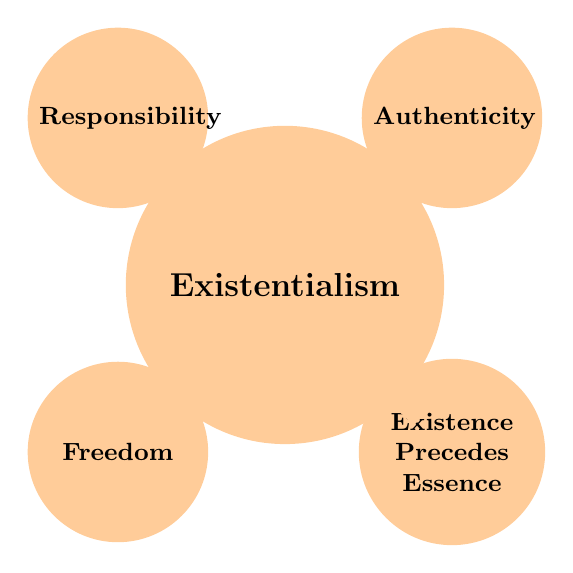
\begin{tikzpicture}[mindmap, grow cyclic, every node/.style=concept, concept color=orange!40, 
			level 1/.append style={level distance=5cm, sibling angle=90},
			level 2/.append style={level distance=3cm, sibling angle=45}, scale = .6]
			
			\node{\textbf{Existentialism}}
			child { node {\textbf{Freedom}} }
			child { node {\textbf{Existence Precedes Essence}} }
			child { node {\textbf{Authenticity}} }
			child { node {\textbf{Responsibility}} };
		\end{tikzpicture}
	\end{frame}
	
	% Slide 8
	\begin{frame}
		\frametitle{Existence Precedes Essence: The Fundamental Existentialist Claim}
		\begin{itemize}
			\item \textbf{Existence precedes essence} means that humans first exist in the world, then create their meaning or purpose through their choices.
			\item This directly challenges traditional philosophical views where humans have a predetermined nature or purpose given by God or metaphysical reality.
			\item For de Beauvoir, this principle grounds her understanding that women are not determined by biology but define themselves through action.
			\item This concept establishes the foundational existentialist commitment to radical freedom and responsibility.
		\end{itemize}
		
		\begin{block}{Traditional View vs. Existentialist View}
			\begin{tabular}{p{0.45\textwidth} | p{0.45\textwidth}}
				\textbf{Traditional View} & \textbf{Existentialist View} \\
				\hline
				Humans have predetermined essence & Humans define themselves through actions \\
				Meaning comes from external sources & Meaning is created by the individual \\
				Nature determines behavior & Freedom shapes identity \\
				Fixed human nature & Open-ended human becoming \\
			\end{tabular}
		\end{block}
	\end{frame}
	
	
	% Slide 9
	\begin{frame}
		\frametitle{Freedom and Responsibility: The Burden of Choice}
		\begin{itemize}
			\item For existentialists like de Beauvoir, humans are \textbf{radically free} to make choices that define who they are.
			\item This freedom is not a gift but a burden, as it comes with complete responsibility for one's choices and their consequences.
			\item De Beauvoir argues that we cannot escape this freedom—even choosing not to choose is itself a choice.
			\item With radical freedom comes \textbf{anguish}, the emotional experience of recognizing the weight of our responsibility.
		\end{itemize}
		
		\begin{alertblock}{The Burden of Freedom}
			De Beauvoir writes in \textit{The Ethics of Ambiguity}: ``Man is condemned to freedom, and from the moment he is thrown into this world, he is responsible for everything he does. It is up to him to give life a meaning.'' This responsibility creates existential anxiety but also opens the possibility for authentic ethical action.
		\end{alertblock}
	\end{frame}
	
	% Slide 10
	\begin{frame}
		\frametitle{Bad Faith: How We Flee from Freedom}
		\begin{itemize}
			\item \textbf{Bad faith} (mauvaise foi) is the existentialist concept describing how humans deny their freedom and responsibility.
			\item People in bad faith pretend they are determined by external factors like biology, social roles, or past events.
			\item De Beauvoir identifies bad faith in women who claim they can't pursue careers because of "feminine nature" or in men who claim "that's just how men are."
			\item Bad faith provides psychological comfort but prevents authentic ethical engagement with life.
		\end{itemize}
		
		\begin{center}
			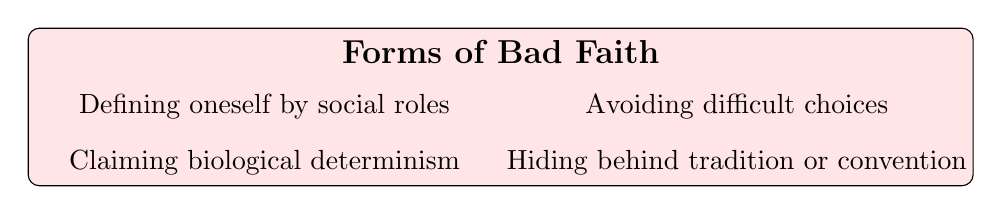
\begin{tikzpicture}
				\draw[rounded corners, fill=red!10] (0,0) rectangle (12,2);
				\node at (6,1.7) {\large \textbf{Forms of Bad Faith}};
				\node at (3,1) {Defining oneself by social roles};
				\node at (9,1) {Avoiding difficult choices};
				\node at (3,0.3) {Claiming biological determinism};
				\node at (9,0.3) {Hiding behind tradition or convention};
			\end{tikzpicture}
		\end{center}
	\end{frame}
	
	% Slide 11
	\begin{frame}
		\frametitle{Authenticity vs. Inauthenticity: Choosing One's Life}
		\begin{itemize}
			\item \textbf{Authenticity} means acknowledging one's freedom and taking responsibility for creating one's self through choices.
			\item An authentic person recognizes that nothing—not God, society, or nature—determines who they must be.
			\item \textbf{Inauthenticity} means living according to external expectations or pretending one has no choice.
			\item For de Beauvoir, the path to ethical living begins with authentic recognition of one's freedom.
		\end{itemize}
		
		\begin{exampleblock}{Examples of Authentic vs. Inauthentic Living}
			\begin{itemize}
				\item \textbf{Authentic:} A woman chooses not to have children because she values other pursuits, fully acknowledging this as her free choice rather than claiming inability or disinterest.
				\item \textbf{Inauthentic:} A person remains in a career they hate but claims they "have no choice" because of financial obligations, rather than acknowledging this as a value decision they continue to make.
			\end{itemize}
		\end{exampleblock}
	\end{frame}
	
	% Slide 12
	\begin{frame}
		\frametitle{The Situation: Freedom Within Constraints}
		\begin{itemize}
			\item De Beauvoir uses the term \textbf{situation} to describe the concrete circumstances that both enable and limit our freedom.
			\item Our situation includes physical facts (body, health), social position (class, gender), historical context, and past choices.
			\item While we don't choose our initial situation, we do choose how we respond to it and what meaning we give it.
			\item Understanding one's situation is essential for exercising authentic freedom rather than abstract, impossible freedom.
		\end{itemize}
		
		\begin{figure}
			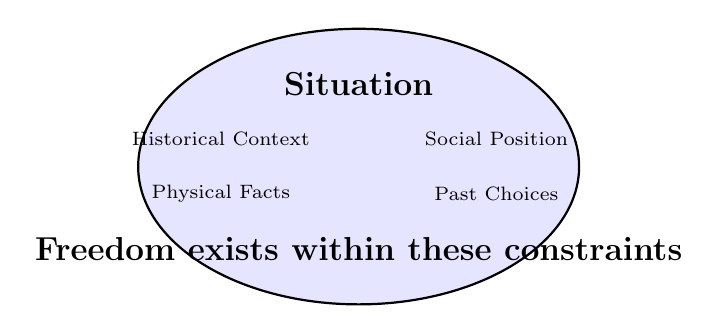
\begin{tikzpicture}[scale = .7]
				\scriptsize
				\draw[thick, fill=blue!10] (0,0) ellipse (4cm and 2.5cm);
				\node at (0,1.5) {\large \textbf{Situation}};
				\node at (-2.5,0.5) {Historical Context};
				\node at (2.5,0.5) {Social Position};
				\node at (-2.5,-0.5) {Physical Facts};
				\node at (2.5,-0.5) {Past Choices};
				\node at (0,-1.5) {\large \textbf{Freedom exists within these constraints}};
			\end{tikzpicture}
		\end{figure}
		\end{frame}
		
		% Slide 13
		\begin{frame}
			\frametitle{De Beauvoir's Contributions to Existentialist Thought}
			\begin{itemize}
				\item De Beauvoir extended existentialist concepts beyond abstract philosophy to address concrete human experiences.
				\item She argued that freedom must be understood in relation to embodied existence and social context, not as pure abstraction.
				\item Her focus on the lived experience of women revealed how existentialist concepts manifest differently across genders.
				\item She developed the concept of \textbf{situated freedom}—the idea that freedom is always exercised within concrete constraints.
			\end{itemize}
			
			\begin{block}{De Beauvoir vs. Sartre}
				\begin{tabular}{p{0.45\textwidth} | p{0.45\textwidth}}
					\textbf{Sartre's Focus} & \textbf{De Beauvoir's Focus} \\
					\hline
					Abstract freedom & Situated freedom \\
					Individual consciousness & Social relations \\
					Ontological questions & Ethical questions \\
					Universal human condition & Gendered experiences \\
				\end{tabular}
			\end{block}
		\end{frame}
		
		% Slide 14
		\begin{frame}
			\frametitle{The Second Sex: Revolutionizing Feminist Philosophy}
			\begin{itemize}
				\item Published in 1949, \textit{The Second Sex} applied existentialist analysis to the situation of women.
				\item The book examines how women have been defined as the \textbf{Other} in relation to men, who are positioned as the Subject.
				\item De Beauvoir analyzes female experience through biology, psychology, history, and myth to reveal how femininity is constructed.
				\item This groundbreaking work laid the theoretical foundation for second-wave feminism and contemporary gender studies.
			\end{itemize}
			
			\begin{alertblock}{Revolutionary Impact}
				\textit{The Second Sex} was immediately controversial upon publication for its frank discussion of women's bodies, sexuality, and oppression. It was placed on the Vatican's list of prohibited books, yet sold over 20,000 copies in its first week. The text remains foundational to feminist philosophy and continues to influence contemporary discussions of gender worldwide.
			\end{alertblock}
		\end{frame}
		
		% Slide 15
		\begin{frame}
			\frametitle{One Is Not Born, But Rather Becomes, A Woman: Social Construction of Gender}
			\begin{itemize}
				\item De Beauvoir's famous statement that ``One is not born, but rather becomes, a woman'' introduced the concept of \textbf{gender as socially constructed}.
				\item She distinguishes between biological sex (physical characteristics) and gender (social roles and expectations).
				\item This insight revealed that what society considers ``feminine'' is not natural or inevitable but learned and enforced.
				\item By showing gender is constructed, de Beauvoir established that women's subordination is not determined by biology but by social structures.
			\end{itemize}
			
			\begin{center}
				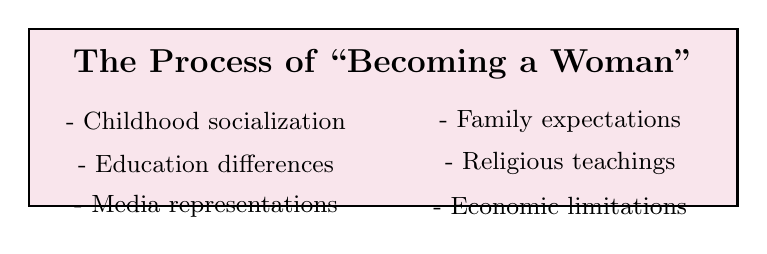
\begin{tikzpicture}[scale = .9]
					\small
					\draw[thick, fill=purple!10] (0,0) rectangle (10,2.5);
					\node[align=center] at (5,2) {\large \textbf{The Process of ``Becoming a Woman''}};
					
					\node[align=left] at (2.5,1.2) {- Childhood socialization};
					\node[align=left] at (2.5,0.6) {- Education differences};
					\node[align=left] at (2.5,0.0) {- Media representations};
					
					\node[align=left] at (7.5,1.2) {- Family expectations};
					\node[align=left] at (7.5,0.6) {- Religious teachings};
					\node[align=left] at (7.5,0.0) {- Economic limitations};
				\end{tikzpicture}
			\end{center}
		\end{frame}
		
		% Slide 16
		\begin{frame}
			\frametitle{The Concept of 'Other': Women as the Second Sex}
			\begin{itemize}
				\item De Beauvoir argues that throughout history, men have positioned themselves as the essential Subject and women as the inessential \textbf{Other}.
				\item This othering process defines woman as relative to man—she is what he is not (emotional vs. rational, passive vs. active).
				\item Unlike other types of otherness (race, class), the relationship between men and women involves intimate proximity and economic dependence.
				\item This concept helps explain why women have often participated in their own subordination, internalizing their status as Other.
			\end{itemize}
			
			\begin{exampleblock}{The Logic of Othering}
				Beauvoir writes: ``He is the Subject, he is the Absolute—she is the Other.'' This dynamic appears in language (mankind includes women, but womankind excludes men), symbolism (God as male), and social structures (male as default, female as exception). This framework reveals that what appears as natural difference is actually a power relation.
			\end{exampleblock}
		\end{frame}
		
		% Slide 17
		\begin{frame}
			\frametitle{Immanence vs. Transcendence: Gendered Experiences of Freedom}
			\begin{itemize}
				\item De Beauvoir uses the terms \textbf{immanence} (being confined within oneself) and \textbf{transcendence} (projecting outward) to analyze gendered experience.
				\item Historically, men have been associated with transcendence—creating, building, exploring, and pursuing projects in the world.
				\item Women have been confined to immanence—maintaining the home, repeating cyclical tasks, and caring for others' bodies.
				\item This division denies women full human freedom, as authentic existence requires both immanence and transcendence.
			\end{itemize}
			
			\begin{center}
				\begin{tabular}{|p{5cm}|p{5cm}|}
					\hline
					\textbf{Immanence (Associated with Femininity)} & \textbf{Transcendence (Associated with Masculinity)} \\
					\hline
					Repetitive, cyclical tasks & Progressive, linear projects \\
					Maintaining life & Creating new things \\
					Private sphere & Public sphere \\
					Body-oriented & Mind-oriented \\
					\hline
				\end{tabular}
			\end{center}
		\end{frame}
		
		% Slide 18
		\begin{frame}
			\frametitle{Myths of Femininity: How Culture Shapes Gender}
			\begin{itemize}
				\item De Beauvoir identifies various \textbf{myths of femininity} that shape cultural expectations of women.
				\item These myths (woman as mother, virgin, temptress, etc.) limit women's freedom by presenting restrictive ideals as natural.
				\item Literature, religion, and psychology have all contributed to these myths that position woman as mysterious Other.
				\item These myths serve to justify women's subordination while making it appear natural and inevitable.
			\end{itemize}
			
			\begin{block}{Key Feminine Myths in Western Culture}
				\scriptsize
				De Beauvoir examines how literature and culture perpetuate contradictory myths of femininity:
				\begin{itemize}
					\item The nurturing, selfless mother (life-giver)
					\item The pure, innocent virgin (moral guardian)
					\item The dangerous temptress (threat to male reason)
					\item The mysterious, unpredictable creature (unknowable Other)
				\end{itemize}
				Each myth limits women's humanity while serving male interests.
			\end{block}
		\end{frame}
		
		% Slide 19
		\begin{frame}
			\frametitle{Lived Experience: The Embodied Reality of Gender}
			\begin{itemize}
				\item De Beauvoir introduces \textbf{lived experience} (l'expérience vécue) as a philosophical concept examining how gender is experienced in the body.
				\item She analyzes experiences like menstruation, sexual initiation, and motherhood to reveal how biological facts acquire social meanings.
				\item These experiences are not merely biological but are shaped by cultural attitudes, economic factors, and social expectations.
				\item Understanding lived experience reveals that biology alone doesn't determine gender—it's how biological facts are interpreted and experienced.
			\end{itemize}
			
			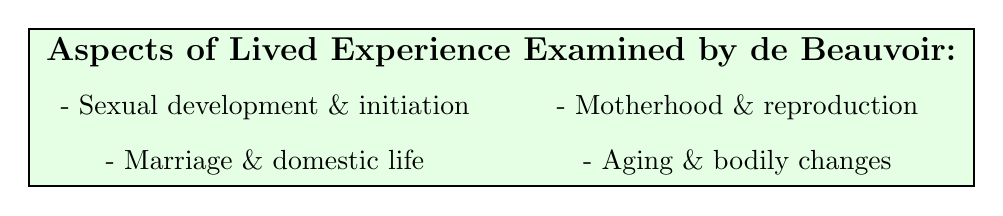
\begin{tikzpicture}
				\draw[thick, fill=green!10] (0,0) rectangle (12,2);
				\node at (6,1.7) {\large \textbf{Aspects of Lived Experience Examined by de Beauvoir:}};
				
				\node[align=left] at (3,1) {- Sexual development \& initiation};
				\node[align=left] at (3,0.3) {- Marriage \& domestic life};
				
				\node[align=left] at (9,1) {- Motherhood \& reproduction};
				\node[align=left] at (9,0.3) {- Aging \& bodily changes};
			\end{tikzpicture}
		\end{frame}
		
		% Slide 20
		\begin{frame}
			\frametitle{Liberation Through Work and Independence}
			\begin{itemize}
				\item De Beauvoir argues that \textbf{economic independence} is essential for women's liberation from subordination.
				\item Meaningful work offers women access to transcendence—the ability to create and engage in the world beyond the home.
				\item She criticizes the double burden many women face: expected to work professionally while still handling all domestic duties.
				\item True liberation requires both economic and psychological independence from men and rejection of imposed feminine ideals.
			\end{itemize}
			
			\begin{alertblock}{The Path to Liberation}
				``It is through gainful employment that woman has traversed most of the distance that separated her from the male; and nothing else can guarantee her liberty in practice.'' De Beauvoir argues that work alone is insufficient—women must also challenge the cultural myths that define femininity and develop a sense of personal agency and independent identity.
			\end{alertblock}
		\end{frame}
		
		% Slide 21
		\begin{frame}
			\frametitle{De Beauvoir's Feminist Legacy: Influence on Modern Feminism}
			\begin{itemize}
				\item De Beauvoir's analysis laid the groundwork for distinguishing between sex and gender, a fundamental concept in contemporary feminism.
				\item Her critique of women's objectification influenced later feminist analyses of media representation and sexual politics.
				\item The concept of situated freedom helped develop intersectional approaches that examine how gender interacts with race, class, and sexuality.
				\item Her insistence that women's liberation requires both material changes and conceptual shifts remains central to feminist theory.
			\end{itemize}
			
			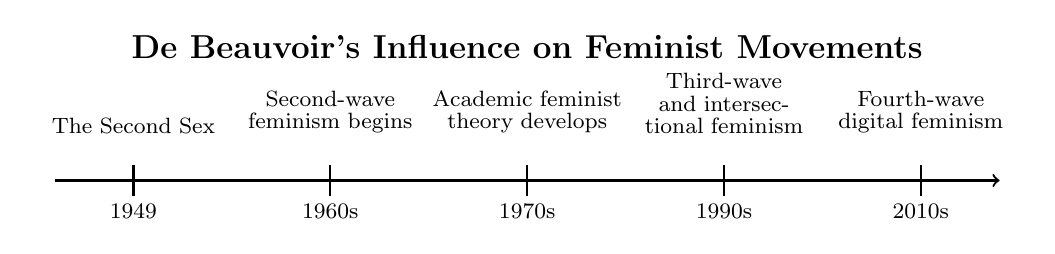
\begin{tikzpicture}
				\scriptsize
				\draw[->, thick] (0,0) -- (12,0);
				\node at (6,1.7) {\large \textbf{De Beauvoir's Influence on Feminist Movements}};
				
				\foreach \x/\year/\event in {
					1/1949/The Second Sex,
					3.5/1960s/Second-wave feminism begins,
					6/1970s/Academic feminist theory develops,
					8.5/1990s/Third-wave and intersectional feminism,
					11/2010s/Fourth-wave digital feminism
				}
				{
					\draw[thick] (\x,-0.2) -- (\x,0.2);
					\node[below] at (\x,-0.2) {\footnotesize \year};
					\node[above, align=center, text width=2.5cm] at (\x,0.5) {\footnotesize \event};
				}
			\end{tikzpicture}
		\end{frame}
		
		% Slide 22
		\begin{frame}
			\frametitle{The Ethics of Ambiguity: An Introduction}
			\begin{itemize}
				\item Published in 1947, \textit{The Ethics of Ambiguity} is de Beauvoir's most systematic work on ethics.
				\item The text develops an existentialist ethics based on the recognition of human freedom and the absence of fixed moral values.
				\item De Beauvoir argues that traditional ethical systems fail because they seek absolute, universal principles that ignore human ambiguity.
				\item The work establishes that authentic ethics must acknowledge the tension between our freedom and our facticity (material limitations).
			\end{itemize}
			
			\begin{exampleblock}{The Central Question}
				How can we establish ethics in a world without absolute values? De Beauvoir addresses the challenge posed by Dostoyevsky's famous question: ``If God is dead, is everything permitted?'' Her answer is that human freedom itself provides the basis for ethics, not through abstract rules but through reciprocal recognition of others' freedom.
			\end{exampleblock}
		\end{frame}
		
		% Slide 23
		\begin{frame}
			\frametitle{Ambiguity as the Human Condition: Neither Pure Object Nor Pure Subject}
			\begin{itemize}
				\item \textbf{Ambiguity} refers to the fundamental tension in human existence: we are both subjects (conscious beings) and objects (physical bodies).
				\item We are simultaneously free to choose and constrained by material conditions we did not choose.
				\item We are both separate individuals and fundamentally connected to others through shared humanity.
				\item De Beauvoir argues that traditional ethics fail because they attempt to resolve this ambiguity rather than recognizing it as the human condition.
			\end{itemize}
			
			\begin{center}
				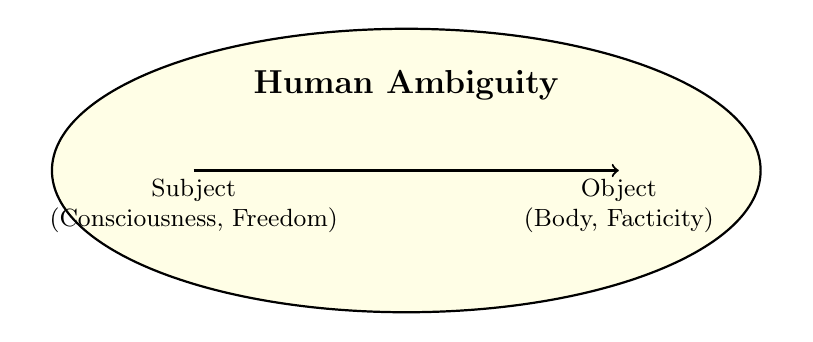
\begin{tikzpicture}[scale = .9]
					\small
					\draw[thick, fill=yellow!10] (0,0) ellipse (5cm and 2cm);
					\node at (0,1.2) {\large \textbf{Human Ambiguity}};
					\draw[thick, ->] (-3,0) -- (3,0);
					\node[text width=4cm, align=center] at (-3,-0.5) {Subject\\ (Consciousness, Freedom)};
					\node[text width=4cm, align=center] at (3,-0.5) {Object\\ (Body, Facticity)};
				\end{tikzpicture}
			\end{center}
		\end{frame}
		
		% Slide 24
		\begin{frame}
			\frametitle{Ethical Freedom: Beyond Nihilism and Absolutism}
			\begin{itemize}
				\item De Beauvoir rejects both \textbf{nihilism} (the belief that no values exist) and \textbf{absolutism} (the belief in fixed, universal values).
				\item She argues that the absence of God or absolute values doesn't mean "everything is permitted"—human freedom itself establishes ethical limits.
				\item We create values through our choices, but these values aren't merely subjective; they arise from our shared human condition.
				\item The recognition of others' freedom becomes the foundation for ethics in a world without absolute principles.
			\end{itemize}
			
			\begin{block}{Between Two Ethical Extremes}
				\scriptsize
				\begin{tabular}{p{0.45\textwidth} | p{0.45\textwidth}}
					\textbf{Ethical Absolutism} & \textbf{Ethical Nihilism} \\
					\hline
					Fixed universal values exist & No values exist at all \\
					Values transcend human choice & Values are purely subjective \\
					Denies human freedom & Renders choices meaningless \\
				\end{tabular}
				
				\vspace{0.3cm}
				De Beauvoir proposes a third way: values emerge from human freedom itself and our recognition of others' freedom.
			\end{block}
		\end{frame}
		
		% Slide 25
		\begin{frame}
			\frametitle{Assuming Our Freedom: The Basis of Ethical Action}
			\begin{itemize}
				\item For de Beauvoir, ethics begins with \textbf{assuming our freedom}—honestly acknowledging that we make choices rather than being determined.
				\item This means recognizing that our actions create who we are; there is no pre-established self that our actions merely express.
				\item Assuming freedom also means accepting the full weight of responsibility for the consequences of our choices.
				\item This authentic assumption of freedom is the foundation for all genuinely ethical action.
			\end{itemize}
			
			\begin{alertblock}{The Fundamental Ethical Choice}
				De Beauvoir writes: "To will oneself free is also to will others free." This means that authentic freedom isn't merely doing what one wants—it's recognizing that one's own freedom is bound up with the freedom of others. This recognition transforms individual freedom into a basis for ethical relations with others.
			\end{alertblock}
		\end{frame}
		
		% Slide 26
		\begin{frame}
			\frametitle{The Serious Person: Avoiding Ethical Responsibility}
			\begin{itemize}
				\item De Beauvoir describes the \textbf{serious person} as someone who escapes freedom by treating values as absolute and external.
				\item The serious person claims to serve pre-established values (God, Nation, Tradition, Family) rather than taking responsibility for creating values.
				\item This attitude allows the serious person to avoid the anxiety of freedom and justify imposing their values on others.
				\item Examples include the religious fundamentalist, the unquestioning patriot, or anyone who claims "this is just how things are."
			\end{itemize}
			
			\begin{exampleblock}{The Danger of Seriousness}
				The serious person claims to serve absolute values but actually uses these values to escape freedom. This perspective is dangerous because it leads to tyranny—since these values are considered absolute, the serious person feels justified in imposing them on others by force. The 20th-century totalitarian regimes demonstrate the ethical and political dangers of the serious attitude.
			\end{exampleblock}
		\end{frame}
		
		% Slide 27
		\begin{frame}
			\frametitle{The Stages of Ethical Development: From Child to Authentic Adult}
			\begin{itemize}
				\item De Beauvoir outlines several ways people relate to freedom, from the child who hasn't yet discovered freedom to the authentic person who fully assumes it.
				\item The \textbf{child} lives in a world of ready-made values, taking the adult world as fixed and given.
				\item The \textbf{sub-human} refuses freedom and lives purely in the moment without projects or values.
				\item The \textbf{serious person} escapes freedom by serving external values.
				\item The \textbf{nihilist} recognizes freedom but responds with destructive denial of all values.
			\end{itemize}
			
			\begin{center}
				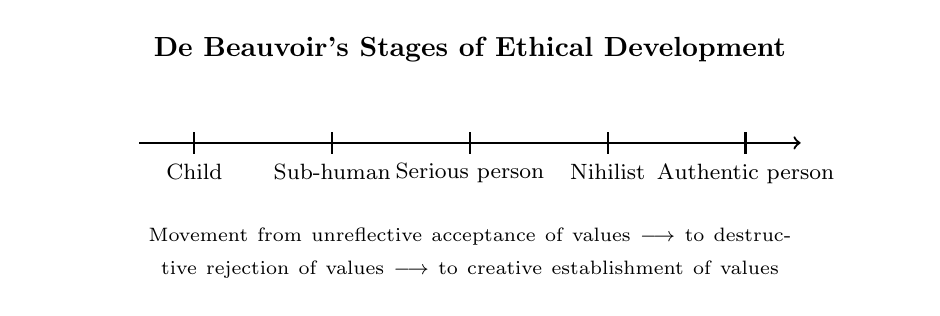
\begin{tikzpicture}[scale = .7]
					\draw[thick, ->] (0,0) -- (12,0);
					\node at (6,1.7) {\normalsize \textbf{De Beauvoir's Stages of Ethical Development}};
					
					\foreach \x/\pos in {
						1/Child,
						3.5/Sub-human,
						6/Serious person,
						8.5/Nihilist,
						11/Authentic person
					}
					{
						\draw[thick] (\x,-0.2) -- (\x,0.2);
						\node[below] at (\x,-0.2) {\footnotesize \pos};
					}
					
					\node[text width=11cm, align=center] at (6,-2) {\scriptsize Movement from unreflective acceptance of values $\longrightarrow$ to destructive rejection of values $\longrightarrow$ to creative establishment of values};
				\end{tikzpicture}
			\end{center}
		\end{frame}
		
		% Slide 28
		\begin{frame}
			\frametitle{Reciprocal Freedom: Ethics in Relation to Others}
			\begin{itemize}
				\item De Beauvoir's ethics centers on the concept of \textbf{reciprocal freedom}—recognizing and supporting others' freedom while exercising our own.
				\item Unlike Sartre's early view that others threaten our freedom, de Beauvoir sees the possibility of ethical relations between free individuals.
				\item We need others to recognize our freedom for it to be concrete and meaningful rather than empty abstraction.
				\item This mutual recognition establishes an ethical bond that isn't based on external authority but on shared commitment to freedom.
			\end{itemize}
			
			\begin{table}
				\begin{tabular}{|p{6cm}|p{6cm}|}
					\hline
					\textbf{Unethical Relation to Others} & \textbf{Ethical Relation to Others} \\
					\hline
					Seeing others as means to an end & Recognizing others as ends in themselves \\
					Imposing one's values on others & Respecting others' freedom to choose \\
					Treating others as objects & Acknowledging others as subjects \\
					Using others for one's projects & Creating shared projects with others \\
					\hline
				\end{tabular}
				\caption{De Beauvoir's View of Interpersonal Ethics}
			\end{table}
		\end{frame}
		
		% Slide 29
		\begin{frame}
			\frametitle{The Appeal to Freedom: Justifying Ethical Choices}
			\begin{itemize}
				\item De Beauvoir introduces the concept of \textbf{the appeal} (l'appel)—the ethical call we make to others to recognize and support our projects.
				\item When we undertake a project (a political cause, artistic creation, etc.), we implicitly appeal to others to acknowledge its value.
				\item This appeal is not coercive but invites others to freely join our project or recognize its legitimacy.
				\item The appeal respects others' freedom while seeking their participation or recognition.
			\end{itemize}
			
			\begin{exampleblock}{Examples of Ethical Appeals}
				The artist creates work that appeals to an audience to recognize its value. The activist appeals to others to join a cause without forcing participation. The teacher appeals to students to freely engage with ideas rather than imposing them. In each case, the appeal invites rather than compels, creating the possibility for shared values that emerge from freedom rather than authority.
			\end{exampleblock}
		\end{frame}
		
		% Slide 30
		\begin{frame}
			\frametitle{Ethics Without Absolutes: Finding Meaning in Ambiguity}
			\begin{itemize}
				\item De Beauvoir argues that ethical life requires embracing ambiguity rather than seeking certainty in absolute rules or values.
				\item We must recognize that moral choices are made in specific situations without the guidance of universal principles.
				\item This doesn't mean ethics is merely subjective—our shared human condition and need for reciprocal freedom provide a basis for judgment.
				\item The authentic ethical person remains open to ambiguity while taking responsibility for creating meaning through choices.
			\end{itemize}
			
			\begin{alertblock}{The Challenge of Ethical Ambiguity}
				``Ethics does not furnish recipes any more than do science and art.'' De Beauvoir emphasizes that there is no formula for ethical action—each situation requires fresh judgment and a willingness to assume responsibility for our choices without the comfort of absolute rules. This makes ethics more demanding but also more authentically human.
			\end{alertblock}
		\end{frame}
		
		% Slide 31
		\begin{frame}
			\frametitle{Beyond Kant: De Beauvoir's Critique of Universal Ethics}
			\begin{itemize}
				\item De Beauvoir critiques Kantian ethics for abstracting moral principles from concrete human situations.
				\item She rejects Kant's \textbf{categorical imperative}—the principle that one should act only according to rules that could be universal laws.
				\item For de Beauvoir, this approach ignores the specific contexts and relationships that give moral choices their meaning.
				\item While Kant seeks universal rules that apply in all cases, de Beauvoir emphasizes situated judgments that respond to particular circumstances.
			\end{itemize}
			
			\begin{tabular}{|p{5.5cm}|p{5.5cm}|}
				\hline
				\textbf{Kantian Ethics} & \textbf{De Beauvoir's Ethics} \\
				\hline
				Universal moral laws & Situated ethical judgments \\
				Duty-based morality & Freedom-based ethics \\
				Rational principles & Embodied decision-making \\
				Abstract moral subject & Socially situated human being \\
				\hline
			\end{tabular}
		\end{frame}
		
		% Slide 32
		\begin{frame}
			\frametitle{Challenging Utilitarianism: Why Happiness Isn't Enough}
			\begin{itemize}
				\item De Beauvoir challenges \textbf{utilitarianism}, which judges actions by whether they produce the greatest happiness for the greatest number.
				\item She argues that utilitarian calculation treats humans as objects whose suffering and happiness can be quantified and compared.
				\item This approach ignores the unique freedom of each person and reduces ethics to a technical problem of maximizing pleasure.
				\item For de Beauvoir, the ethical goal isn't happiness but freedom—the opportunity to create meaning through authentic choices.
			\end{itemize}
			
			\begin{block}{De Beauvoir's Critique of Utilitarian Ethics}
				\scriptsize
				\begin{columns}
					\begin{column}{0.48\textwidth}
						\begin{itemize}
							\item Reduces humans to calculable quantities
							\item Treats happiness as a simple, measurable good
							\item Ignores the value of freedom itself
							\item Can justify sacrificing individuals for majority
						\end{itemize}
					\end{column}
					\begin{column}{0.48\textwidth}
						\begin{itemize}
							\item Establishes external criterion of "utility"
							\item Makes ethics a technical problem
							\item Overlooks meaning beyond pleasure/pain
							\item Disregards ethical importance of intention
						\end{itemize}
					\end{column}
				\end{columns}
			\end{block}
		\end{frame}
	
	% Slide 33
	\begin{frame}
		\frametitle{Marxism and Ethics: De Beauvoir's Critical Engagement}
		\begin{itemize}
			\item De Beauvoir engages with \textbf{Marxism}, appreciating its analysis of material conditions while criticizing its deterministic aspects.
			\item She agrees with Marx that economic conditions shape our possibilities but rejects the idea that history follows predetermined laws.
			\item De Beauvoir critiques Marxist ethics for sometimes sacrificing present individuals for an abstract future society.
			\item She argues that revolution must be grounded in ethical commitment to freedom, not just economic analysis.
		\end{itemize}
		
		\begin{block}{De Beauvoir and Marx: Points of Agreement and Disagreement}
			\begin{tabular}{p{0.45\textwidth} | p{0.45\textwidth}}
				\textbf{Points of Agreement} & \textbf{Points of Disagreement} \\
				\hline
				Importance of material conditions & Economic determinism \\
				Critique of bourgeois individualism & Subordination of ethics to politics \\
				Need for social transformation & Sacrifice of present for future \\
				Analysis of exploitation & Belief in historical inevitability \\
			\end{tabular}
		\end{block}
	\end{frame}
	
	% Slide 34
	\begin{frame}
		\frametitle{Existentialism vs. Traditional Religious Ethics}
		\begin{itemize}
			\item De Beauvoir contrasts existentialist ethics with \textbf{religious ethics} that derive moral principles from divine authority.
			\item She argues that religious ethics often avoid ambiguity by establishing absolute rules that followers must obey.
			\item While religious ethics provides certainty, it can lead to the "serious attitude" that escapes responsibility for creating values.
			\item For de Beauvoir, authentic ethics requires assuming responsibility rather than following pre-established commands.
		\end{itemize}
		
		\begin{table}
			\begin{tabular}{|p{5.5cm}|p{5.5cm}|}
				\hline
				\multicolumn{2}{|c|}{\textbf{Religious Ethics vs. Existentialist Ethics}} \\
				\hline
				\textbf{Religious Ethics:} & \textbf{Existentialist Ethics:} \\
				Source of value is external & Source of value is human freedom \\
				(God, scripture, tradition) & (personal choice, responsibility) \\
				\hline
			\end{tabular}
		\end{table}
	\end{frame}
	
	% Slide 35
	\begin{frame}
		\frametitle{Situational Ethics: Context, Freedom, and Ethical Choice}
		\begin{itemize}
			\item De Beauvoir argues for a \textbf{situational ethics} that considers the specific context of each moral decision.
			\item She rejects both abstract moral principles and complete moral relativism in favor of contextualized judgment.
			\item Each ethical situation must be evaluated in terms of its particular features, the people involved, and material conditions.
			\item This approach recognizes that ethical choices occur in concrete situations with specific constraints and possibilities.
		\end{itemize}
		
		\begin{exampleblock}{Ethics in Context: A Case Example}
			De Beauvoir discusses violence as an ethical dilemma: Is violence ever justified? Rather than offering an absolute yes or no, she argues that violence must be evaluated in specific situations. Violence in self-defense differs from violence to oppress others. Violence as part of liberation movements differs from violence that maintains oppression. The ethical evaluation depends on whether the violence expands or diminishes human freedom in that specific context.
		\end{exampleblock}
	\end{frame}
	
	% Slide 36
	\begin{frame}
		\frametitle{De Beauvoir's Ethical Legacy: Influence on Contemporary Thought}
		\begin{itemize}
			\item De Beauvoir's ethics has influenced diverse philosophical movements including feminist ethics, existential psychotherapy, and political theory.
			\item Her emphasis on situated freedom anticipates contemporary approaches that examine how identity factors affect ethical choices.
			\item Her analysis of gender demonstrates how abstract ethical principles often ignore the specific situations of marginalized groups.
			\item De Beauvoir's integrative approach—connecting philosophy, literature, and politics—continues to inspire interdisciplinary ethical thinking.
		\end{itemize}
		
		\begin{alertblock}{Contemporary Relevance}
			De Beauvoir's ethics remains highly relevant to contemporary issues: Her critique of abstract universalism speaks to debates about global ethics across cultural differences. Her analysis of how gender affects ethical experience informs feminist ethics of care. Her emphasis on situated judgment helps address complex bioethical dilemmas. Her thought continues to evolve through the work of philosophers like Judith Butler, Martha Nussbaum, and Iris Marion Young.
		\end{alertblock}
	\end{frame}
	
	
	% Slide 37
	\begin{frame}
		\frametitle{Discussion Questions: Applying Existentialist Ethics}
		\begin{block}{Freedom and Responsibility in Your Life}
			\begin{itemize}
				\item Think of a significant choice you've made recently. How did this choice define who you are becoming? In what ways did you take responsibility for this choice?
				\item De Beauvoir argues that we often flee from freedom through "bad faith." Can you identify instances where you or others have attributed choices to external factors ("That's just how things are") rather than acknowledging freedom?
				\item How does your "situation" (your specific circumstances of gender, economic position, family background, etc.) both limit and enable your freedom? Give concrete examples.
				\item Do you agree with de Beauvoir that there are no absolute moral rules? How do you make ethical decisions without such guidelines?
			\end{itemize}
		\end{block}
		
	\end{frame}
	
	% Slide 38
	\begin{frame}
		\frametitle{Discussion Questions: De Beauvoir's Feminism Today}
		\begin{block}{Gender and Social Construction}
			\begin{itemize}
				\item De Beauvoir famously stated that "One is not born, but rather becomes, a woman." Reflect on the ways you have been shaped by gender expectations in your own life. What messages about gender did you receive growing up?
				\item Consider de Beauvoir's concepts of "immanence" and "transcendence." Do you see these gendered patterns in contemporary life? Give examples from school, work, or family.
				\item How might social media both reinforce and challenge the "myths of femininity" that de Beauvoir critiqued? Consider specific platforms and their impact.
				\item De Beauvoir argued that economic independence is crucial for women's freedom. How relevant is this idea today? Does financial independence ensure freedom?
			\end{itemize}
		\end{block}
		
	\end{frame}
\end{document}
